
\section{Model Development} 

Previous studies \cite{Ans2013} suggest that feedback through supply-demand price mechanisms will have only limited impact on fossil fuel companies. This is due to the fact, that only approximately 15 \% of investors invest subject to socially responsible guidelines \cite{SIF2014Report} and that divested holdings are, especially in liquid markets, very likely to quickly find their way to less responsible investors. \\
Also, as long as the physical capital relying on fossil fuels already exists, economic reasoning follows that it will be used as long as variable costs are covered.
Therefore, a general economic shift from dirty to clean technology needs changes in investment in physical capital or a political imperative mandated by a (qualified) majority. Therefore, I consider a model focussing on savings and investment decisions appropriate to investigate the possible dynamics of an economic transition towards fossil resource independent technologies.\\
In the following I propose a preliminary scheme of such a model.

\begin{figure}[t]
	\centering
	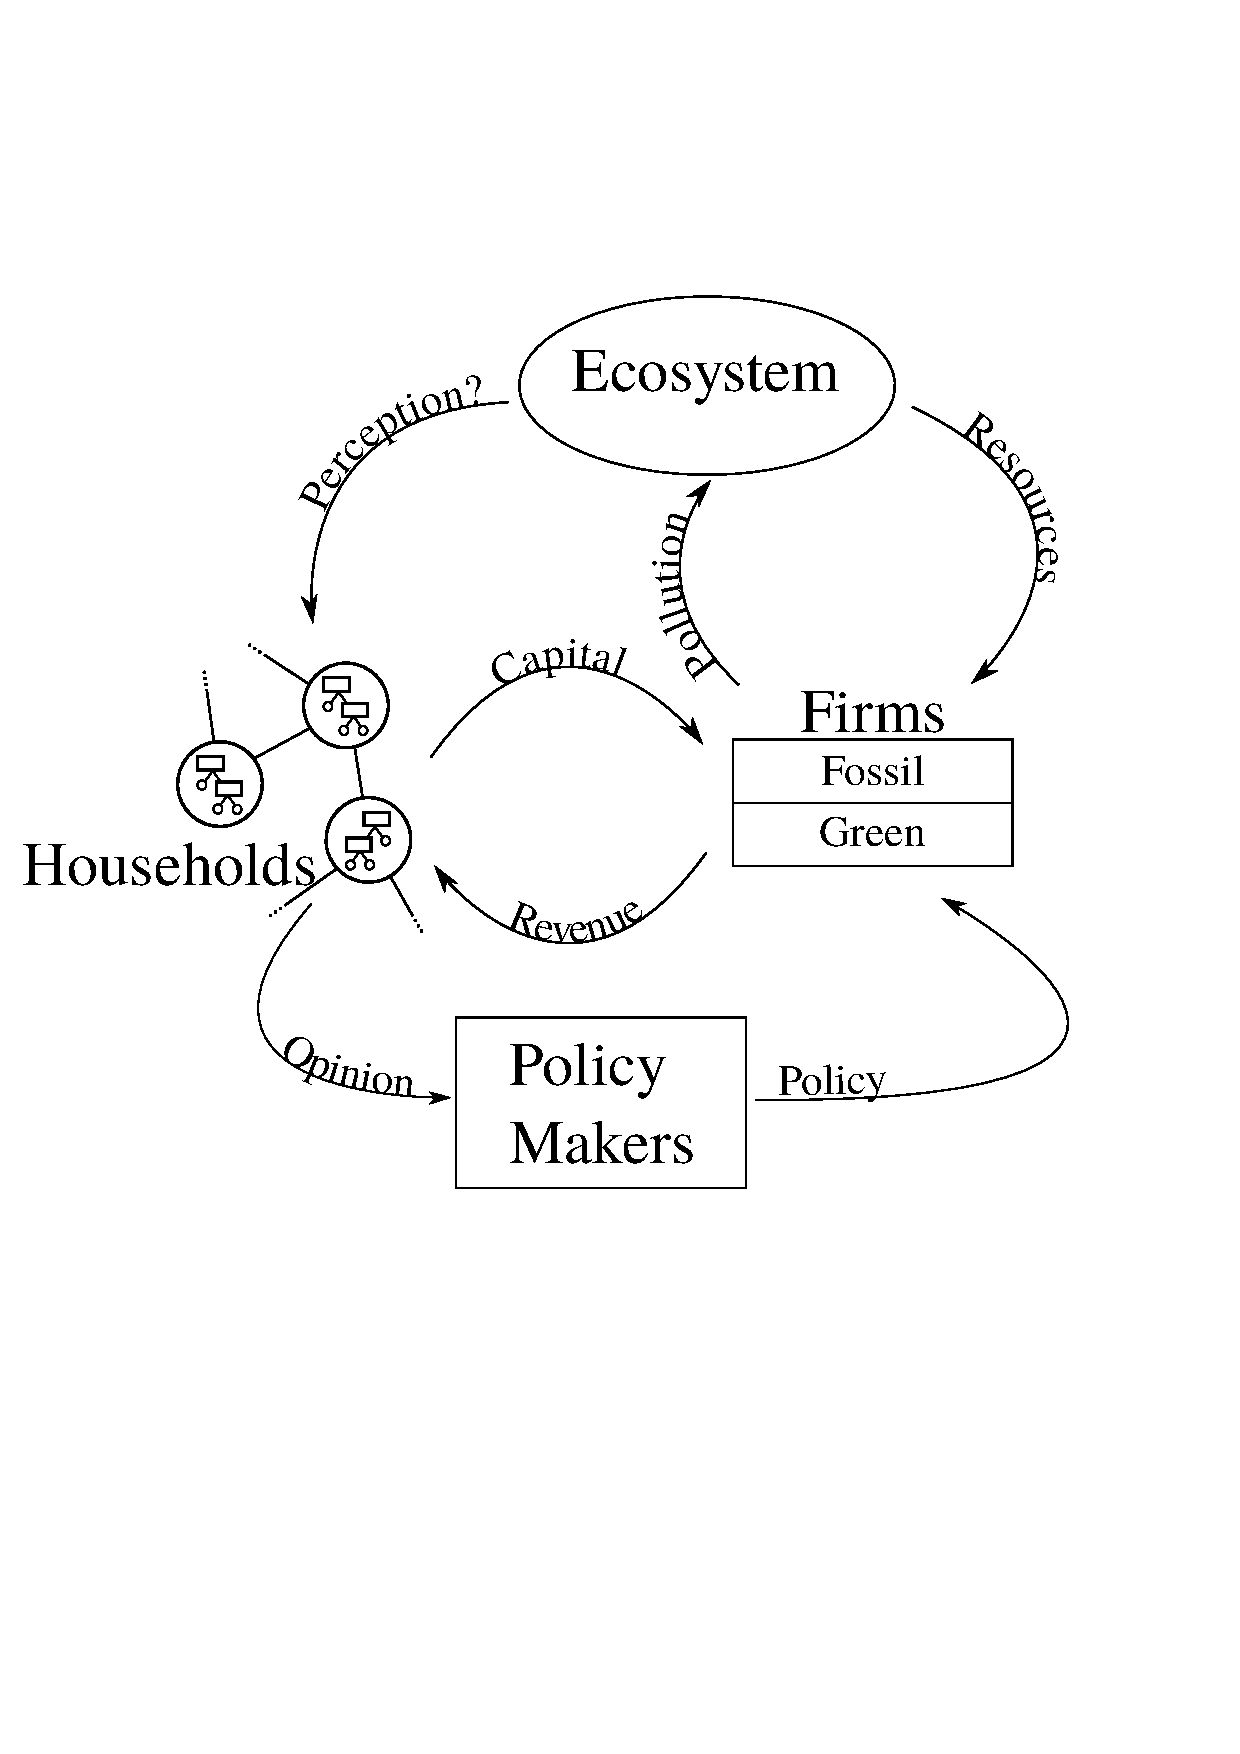
\includegraphics[width =.7 \textwidth]{figures/Model_Scheme.pdf}
	\caption{Schematic sketch of the model including four major components: Households, Firms (grouped by sector), Ecosystem and optional Policy makers.}
	\label{fig:model}
\end{figure}

\subsection{Economic Production}
\label{sec:model_description}

Out model consists of two sectors for production and a set of heterogeneous households that interact via an adaptive complex social network. The production sectors employ different technology. We call them the \textit{clean} and the \textit{dirty} sector for illustrative clarity. The heterogeneous households in the model provide capital $K$ and labor $L$ to both sectors.
In addition, the production technology in the dirty sector depends on the input of an exhaustible (fossil) energy-resource $R$ that is used up in the process. We assume that the technology in the dirty sector is fully developed and adequately described in terms of the total factor productivity. 
Price elasticities of demand for fossil fuel are evidently low in real economies \cite{IMF2011, Hosslinger2017, Labandeira2017}, even with the choice between alternative technologies factored in. We approximate this by setting the elasticity of substitution between the fossil resource and the pair of capital and labor to zero in the dirty sector. This is also in line with contemporary critique of the neoclassical growth models \cite{Daly1997,georgescu1975energy,georgescu1979comments, Ayres2007, Ayres2013} that highlights the generally assumed substitutability of natural resources in production as being physically implausible and lacking empirical evidence.

We acknowledge the common argument for substitutability between capital, labor and energy resources due to a shift in the output of economic production from manufacturing to services and would argue that our model pictures this in a shift of economic production from the dirty sector to the clean one which is described in the following.

The clean sector represents a circular economy in which the output of final goods depends on the machinery, knowledge and effort used in its production and is not limited by entropy laws or resource scarcity on the timescale under consideration. The technology $C$ used in the clean sector is assumed to be still in development and is therefore explicitly modeled.
Following \cite{argote1990learning}, we model technological process as learning by doing according to Wright's law \cite{wright1936factors, Nagy2013} with a one-factor learning curve. We assume that $C$ is proportional to cumulative production but also depreciates with a constant rate $\chi$. Depreciation can be regarded as a human capital effect that leads to knowledge depreciation over time \cite{Kahouli-Brahmi2008}. This is also in line with the empirically observed decrease in learning rates for maturing technologies \cite{argote1990learning}

\begin{equation}
	\dot{C} = Y_c - \chi C.
	\label{eq:learning_by_doing}
\end{equation}

Capital, labor and technology/knowledge are assumed to be mutual substitutes. To satisfy these requirements, we use the following production functions:
\begin{align}
	Y_c &= b_c C^{\gamma} L_c^{\alpha_c}K_c^{\beta_c}, \label{eq:clean_production} \\
	Y_d &= {\mathrm min}\left( b_d L_d^{\alpha_d}K_d^{\beta_d}, e R \right), \label{eq:dirty_production}
\end{align}
Subscripts $c$ and $d$ denote the clean and dirty sector respectively, $L_c$ and $L_d$ are labor shares, $\alpha$ and $\beta$ are elasticities of the respective input factors and $b_c$ and $b_d$ are the total factor productivity and $K_c$ and $K_d$ are the capital stocks for the respective sector. Measuring unit production cost in the number of working hours as in the original study by Wright \cite{wright1936factors}, $\gamma$ is equivalent the elasticity of learning by doing in the clean sector as outlined in \cite{Kahouli-Brahmi2008}.

We assume efficient an usage of resources in the dirty sector, such that
\begin{equation}
    b_d L_d^{\alpha_d}K_d^{\beta_d} = e R
    \label{eq:efficient_dirty_resources}
\end{equation}
where $1/e$ is the resource intensity of the sector. The usage of the fossil resource $R$ depletes a geological resource stock $G$ with the initial stock $G(t=0) = G_0$:
\begin{equation}
    \dot{G} = -R. 
    \label{eq:resource_depletion}
\end{equation} 
In line with the assumptions common in the literature \cite{Dasgupta1974, Perman2003}, the total cost $c_R$ for the usage of the fossil resource depends on the resource use $R$ and the remaining fossil resource stock $G$ such that $\partial c_R / \partial R >0$ and $\partial c_R / \partial G < 0$. We chose the specific form to be
\begin{equation}
	c_R = b_R R^{\rho}\left( \frac{G_0}{G} \right)^{\mu}; \quad \rho \geq 1, \quad \mu > 0,
	\label{eq:resource_cost}
\end{equation}
such that at some point $\partial Y_d / \partial R < \partial c_R / \partial R$ to take into account that some part of the resource is not economic, e.g. its marginal cost exceeds its marginal productivity.
Perfect labor mobility and competition for labor between the two sectors lead to an equilibrium wage $w$ that equals the marginal return for labor:
\begin{equation}
	w = \frac{\partial Y_c}{\partial L_c} = \frac{\partial Y_d}{\partial L_d} - \frac{\partial c_R}{\partial L_d}
	\label{eq:equilibrium_wage}
\end{equation}
with the sum of the labor shares equal to the total amount of labor available:
\begin{equation}
	L_c + L_d = L.
	\label{eq:population}
\end{equation}
We assume physical capital to be specific to the technology employed such that it can only be used in the sector that it has been invested in originally, resulting in separate capital markets for the two sectors. We assume these capital markets to be fully competitive resulting in capital rents equal to marginal productivity:
\begin{align}
	r_c &= \frac{\partial Y_c}{\partial K_c} \label{eq:clean_capital_rent}\\
	r_d &= \frac{\partial Y_d}{\partial K_d} - \frac{\partial c_R}{\partial K_d} \label{eq:dirty_capital_rent}
\end{align}

\subsection{Investment Decision Making}
We model households as bounded rational decision makers \cite{simon1972theories, simon1982models, gigerenzer2002bounded}.
That is, households take their investment decisions, i.e. whether to invest their savings in the clean or the dirty sector, not by forming rational expectations \cite{Evans2006, Kirman2014} but by A) using \emph{heuristic decision strategies} to make robust decisions with sparce information and with limited computational work and B) engaging in \emph{social learning} \cite{bandura1977} to obtain successful decision strategies \cite{Traulsen2010} with reasonable effort.

% Why use Fast and Frugal heuristics for decision making?
Regarding individual decision making, there is ample evidence that real investors rather use a diverse set of heuristic strategies to make investment decisions \cite{Gigerenzer2018} and researchers in the field strongly suggest to consider these so called \emph{Fast and Frugal heuristic} decision models as a complementary alternative to established probabilistic and optimizing decision models. 
In general, Fast and Frugal Heuristics are described in terms of three building blocks; one for information search, one for stopping information search and one for evaluating the available information and drawing a conclusion from it.
We use a decision heuristic called \emph{Take The Best} that is observed to be frequently used in situations where individuals need to decide between one of two options that are comparable in different aspects [CITE]. 
Take the Best has the following building blocks: 1) Search through cues in a predefined order, 2) stop as soon as one cue discriminates between the two options, 3) chose the option with the preferable value on the discriminating cue. \\
This requires a so called \textit{cue order} e.g.\ a hierarchy of validity for the pieces of information that are considered relevant for the decision. \\

% How these heuristics can be interpreted in this context.
Research on perception and decision making in psychology where the concept of Fast and Frugal heuristics was developed usually considers inferential decisions (since they have true and false outcomes and can therefore be benchmarked and evaluated statistically).\\
Nevertheless, Heuristic decision making is a reasonable tool for preferential decisions as well. Although in this context the interpretation of cue orders would be different - namely, they would rather be considered as norms or underlying preferences that apply to the context of the decision. \\
The case of savings decisions that is considered in this model poses an intermediate case between preferential and inferential decisions for a number of reasons. First, there is no immediate feedback on savings decisions, since the return on investment depends on the future development of the economic system which again depends on the savings decisions of all other households and second, we assume that households do not only consider financial but also moral grounds for their savings decisions.
Additionally, I argue that imitation of peers is not only an efficient learning strategy in many situations but also a value in its own - especially if the question is to some extend ethical. 

% Heuristics can be learned from others. This is why we model social learning.
Nevertheless, some strategies are suspected to have more profitable long term results then others as the performance of this decision heuristic depends on the order of the sequence of cues [CITE]. Empirical evidence shows that if participants in an experiment are allowed to share information about their cue orders and respective performance, they do so and thereby greatly increase the speed of learning of cue orders that fit their decision environment compared to individual trial and error reinforcement learning [CITE]. Therefore, we use social learning among households to determine the particular cue order that determines their investment decision making.

% As the outcomes of social learning depend on network topology, we model topology endogenously.
As the outcomes of social learning crucially depend on the structural properties of the complex network of social ties amongst the households \cite{Barkoczi2016}, we model the adaptive formation of this social network endogenously.
A well established principle for the emergence of structured ties in social networks is homophily, i.e. the tendency that similar individuals are linked \cite{McPherson2007, Centola2007, Centola2011}. Especially the concept of value homophily \cite{McPherson2007} is in line with the interpretation of cue orders above not only as a means to the end of making profitable investment decisions but also as an expression of identity and beliefs with regards to clean technology.
The following model specification uses social learning in combination with endogenous network adaptation based on homophily to model the changes in heuristic decision strategies that households use to make investment decisions.

% How I do this technically (Individual Household earnings and investment)
We model $N$ heterogeneous households denoted with the index $i$ as owners of one unit of labor $L^{(i)} = L/N$ and capital $K_c^{(i)}$ and $K_d^{(i)}$ in the clean and dirty economic sector respectively.
Households generate an income $I^{(i)}$ from their labor and capital income which they use for consumption $F^{(i)}$ and savings $I^{(i)}$:
\begin{align}
	I^{(i)} &= w L^{(i)} + r_c K_c^{(i)} + r_d K_d^{(i)}, \label{eq:household_income} \\
	F^{(i)} &= (1-s) I^{(i)}, \label{eq:consumption} \\
	S^{(i)} &= s I^{(i)}. \label{eq:savings}
\end{align}
A binary decision parameter $o_i \in [c,d]$ denotes the sector in which the households decide to invest. As motivated above, we model decision making that is driven by three processes: Heuristic decision making via the Take The Best heuristic, social learning via the imitation of successful cue orders and homophily towards individuals exhibiting the same beliefs as represented by its cue order. \par

% How I do this technically (Heuristic and cue order here)
Concerning the information that households use to make their investment decisions, they are assumed to have no knowledge of the future, e.g.\ they make decisions based solely upon information about the past and present. Possible sources of information are economic indicators such as capital rents in both sectors $r_c$ and $r_d$ and their trends $\dot{r}_c$ and $\dot{r}_d$ as well as observable behavior of other households that they are connected to via the social network and subjective beliefs of superiority of one over the other sector that are not explained by other factors.\\
Each household is characterized by a cue order $O$ containing some or all of the above cues in a specific order. At each time, it uses the Take the Best Heuristic with this cue order to evaluate the information that is available and make an investment decision accordingly.
\par

% How I do this technically (social learning of cue orders)
We describe households as the nodes in a graph of acquaintance relations. Households get active at a constant rate $1/\tau$. When a household $i$ becomes active, it interacts with one of its acquaintances $j$ chosen at random. If they follow the same strategy, i.e. they share the same cue order $O$, nothing happens. If they follow a different strategy, i.e. they differ in their cue order, one of two actions can happen:
\begin{itemize}
	\item Homophilic network adaptation: with probability $\varphi$, the households end their relation and household $i$ connects to another household $k$, that has the same cue order. 
	\item Imitation: with probability $1-\varphi$, household $i$ engages in social learning i.e. it imitates the cue order of household $j$ with a probability $p_{ji}$ that increases with their difference in income.
\end{itemize}
We follow previous results on human strategy updating in repeated interactions \cite{Traulsen2010}, when we assume the imitation probability as a monotonously increasing function of the relative difference in consumption between both households:
\begin{equation}
	p_{ji} =  \left(1 + \exp \left(- \frac{a(F^{(i)} - F^{(j)})}{F^{(i)} + F^{(j)}} \right) \right)^{-1}.
    \label{eq:imitation_probability}
\end{equation}
As opposed to the absolute difference in the original study \cite{Traulsen2010}, the probability in our model depends on relative differences. This dependence on relative differences in per household quantities is crucial for approximation methods as we will discuss later at the end of \ref{sec:large_system_limit}.
We set $a = 8$ to conform to their empirical evidence.
We model strategy exploration as a fraction $\varepsilon$ of events that are random, e.g. rewiring to a random other household or randomly choosing one of the possible cue orders with equal probability.

% Yes, we know, this is only one of the many possible ways to implement such a model.
We acknowledge the fact that different model specifications are possible and interesting.
For instance, we only consider fixed savings rates and the decision between two capital assets and leave the investigation of households setting their savings rates individually to another study \cite{Asano2018}.
Also, this framework might as well be used to test other strategies for decision making such as tallying or pure social learning similar to the approach taken by Barkoczi \cite{Barkoczi2013a}, \cite{Barkoczi2016}

% Capital accumulation of individual households given the model assumptions above.
Given the savings decisions of the individual households, and assuming equal capital depreciation rates $\kappa$ in both sectors, the time development of their capital holdings is given by
\begin{align}
  \dot{K}_c^{(i)} =& \delta_{o_ic} \left( r_c K_c^{(i)} + r_d K_d^{(i)} + w L_i \right) - \kappa K_c^{(i)}, \label{eq:clean_investment}\\
  \dot{K}_d^{(i)} =& \delta_{o_id} \left( r_c K_c^{(i)} + r_d K_d^{(i)} + w L_i \right) - \kappa K_d^{(i)}, \label{eq:dirty_investment}
\end{align}

where $\delta_{ij}$ is the Kronecker Delta. The total capital stocks in the two sectors are made up of the sum of the individual capital stocks as
\begin{equation}
K_j = \sum_i^N K_j^{(i)} = N k_j,
\end{equation}
where $k_j$ is the average per household capital stock of a given capital type.

\subsection{Policy Makers}
\textit{Optional:} \\
Policy makers can implement some carbon tax or carbon cap on economy to incentivize green development. The implementation of such measure depends on the prevalence of opinions amongst voters (are investors a representative sample of voters?) and might be appropriately implemented by a Poisson distributed random variable.

% This is the model. Now lets see what it does.
With the model specifications from above, the parametrization in Tab.~\ref{tab:Parameter_list} and appropriate initial conditions for the dynamic variables, the model can be numerically simulated.
For this, we implemented the dynamics in the multi-purpose programming language python. The implementation of the agent based model, as well as the numerical analysis using the approximation methods described in the following are available on github in \cite{kolb2018}.
In the following, I discuss the technical details ans specification of this implementation.


\begin{table}[t]
	\centering
	\begin{tabular}{r|l}
		Variable & Description \\\hline
		$K^{(i)}_c(t)$ & clean capital of household $i$ \\
		$K^{(i)}_d(t)$ & dirty capital of household $i$ \\
		$G(t)$ & Geological carbon stock \\
                $C(t)$ & Knowledge stock in the clean sector \\
		$O_i(t)$ & opinion/cue order of household $i$ \\
		$o_i(t) \in [c,d]$ & investment decision of household $i$ 
	\end{tabular}
	\caption{Variables of the model with description.}
	\label{tab:independent_variables}
\end{table}
 
\begin{table}[t]
	\centering
	\begin{tabular}{r|l}
		Variable & Description \\\hline
		$w(t)$   & Wage rate, \\
		$r_j(t)$ & Capital return rate in sector $j$, \\
		$c_R(t)$ & Fossil resource extraction cost, \\
		$Y_j(t)$ & Output of sector, $j$ \\
		$L_j(t)$ & total labor employed in sector $j$, \\
		$K_j(t)$ & Total capital employed in sector $j$, \\
		$R(t)$ & Rate of resource uptake of dirty sector. \\
	\end{tabular}
	\caption{Variables of the model with description.}
	\label{tab:derived_variables}
 \end{table}

\begin{table}[t]
	\centering
	\begin{tabular}{r|l}
		Parameter & Description \\\hline
		$b_j$ & total factor productivity in sector $j$ \\
		$\alpha_j$ & elasticity of labor in sector $j$ \\
		$\beta_j$ & elasticity of capital in sector $j$ \\
                $\gamma$ & Elasticity of knowledge in the clean sector\\
		$\rho$ & Elasticity of fossil resource in resource extraction costs \\
		$b_R$ & resource uptake efficiency for fossil resource \\
		$L$ & Total population \\
		$s$ & savings rate \\
		$\delta $ & Capital depreciation rate \\
                $\chi$ & Knowledge depreciation rate\\
		$\tau$ & activity rate of households \\
		$\varphi$ & rewiring probability given an interaction event
	\end{tabular}
	\caption{Parameters of the model with description.}
	\label{tab:parameters}
\end{table}
 
\section{Implementation} 

For simplicity, I assume equal labor elasticities in both sectors ($\alpha_c = \alpha_d$), linear resource extraction costs ($\rho=1$) and no profits e.g. $\alpha_j + \beta_j = 1$.\\

The conditions for labor shares and wages as well as optimal resource uptake pose algebraic constraints for the system of ordinary differential equations that describe the dynamics of the capital stocks $\dot{K}_i^{(j)}$, the resource stock $\dot{G}$ and the dynamics of the knowledge stock in the clean sector $\dot{C}$. In order to solve these differential equations more efficiently, one can solve these algebraic constraints analytically.


\subsection{Calculation of wages, resource uptake and capital rent}

To calculate the labor shares $L_c$ and $L_d$ as well as the wages in the two sectors, we use equations \eqref{eq:resource_cost} and \eqref{eq:equilibrium_wage} and for simplicity assume $\rho=1$ and $\mu=2$. We also assume equal labor elasticities in both sectors $\alpha_d = \alpha_c = \alpha$ resulting in
\begin{align}
	w &= \frac{\partial Y_d}{\partial L_d} - \frac{\partial c_R}{\partial L_d} \nonumber \\
	&= \frac{\partial Y_d}{\partial L_d} - \frac{\partial c_R}{\partial R} \frac{\partial R}{\partial L_d} \nonumber = \frac{\partial Y_d}{\partial L_d} - \frac{\partial c_R}{\partial R} \frac{\partial}{\partial L_d} \frac{Y_d}{e} \nonumber \\
	&= \frac{\partial Y_d}{\partial L_d} - b_R\frac{G_0^2}{G^2} \frac{\partial}{\partial L_d} \frac{Y_d}{e} = b_d \alpha L_d^{\alpha-1} K_d^{\beta_d}\left( 1-\frac{b_R}{e}\frac{G_0^2}{G^2} \right)
	\label{eq:dirty_wages}
\end{align}
for the dirty sector and
\begin{equation}
	w = b_c \alpha L_c^{\alpha-1} K_c^{\beta_c} C^{\gamma}
	\label{eq:clean_wages}
\end{equation}
for the clean sector. Combining these results via equation \eqref{eq:population} results in
\begin{equation}
	L = \left( \frac{w}{\alpha} \right)^{\frac{1}{\alpha-1}}\left( \left( b_c K_c^{\beta_c}C^{\gamma} \right)^{\frac{1}{1-\alpha}} + \left( b_d K_d^{\beta_d} \left( 1 - \frac{b_R}{e}\frac{G_0^2}{G^2} \right) \right)^{\frac{1}{1-\alpha}} \right).
\end{equation}
Substituting 
\begin{equation}
	X_c = (b_c K_c^{\beta_c}C^{\gamma})^{\frac{1}{1-\alpha}}, \qquad X_d = (b_d K_d^{\beta_d})^{\frac{1}{1-\alpha}}, \qquad X_R = \left( 1 - \frac{b_R}{e}\frac{G_0^2}{G^2} \right)^{\frac{1}{1-\alpha}}
	\label{eq:substitutions}
\end{equation}
and solving for $w$ yields:
\begin{equation}
	w = \alpha L^{\alpha-1}\left( X_c + X_d X_R \right)^{1-\alpha}.
	\label{eq:wage_result}
\end{equation}
Plugging \eqref{eq:wage_result} into equations \eqref{eq:dirty_wages} and \eqref{eq:clean_wages} results in 
\begin{align}
	L_c &= L \frac{X_c}{X_c + X_d X_R}, \label{eq:clean_labor} \\
	L_d &= L \frac{X_d X_R}{X_c + X_d X_R} \label{eq:dirty_labor}
\end{align}
for the labor shares and plugging this into \eqref{eq:efficient_dirty_resources} results in
\begin{equation}
	R = \frac{b_d}{e}K_d^{\beta_d}L^{\alpha}\left( \frac{X_d X_R}{X_c + X_d X_R} \right)^{\alpha}
	\label{eq:R_result}
\end{equation}
for the use of the fossil resource. Using the results for $L_c$ and $L_d$ together with equations \eqref{eq:clean_capital_rent} and \eqref{eq:dirty_capital_rent}, the return rates on capital result in
\begin{align}
	r_c &= \frac{\beta_c}{K_c}X_c L^{\alpha}\left( X_c + X_d X_R \right)^{-\alpha}, \label{eq:r_c_result}\\
	r_d &= \frac{\beta_d}{K_d}\left(X_d X_R\right) L^{\alpha}\left( X_c + X_d X_R \right)^{-\alpha}. \label{eq:r_d_result}
\end{align}

It is also worth noting that if we assume constant returns to scale with respect to capital and labor, e.g.

\begin{equation}
	\beta_c = \beta_d = 1-\alpha,
	\label{eq:elasticities_restriction}
\end{equation}

(even though it is not necessary for our method) this results in zero profits in both sectors:
\begin{align}
	Y_c &= w L_c + r_c K_c, \nonumber \\
	Y_d &= w L_d + r_d K_d + c_R. \nonumber
\end{align}

%It is also worth noting, that the assumption of zero profits, e.g.
%\begin{align}
%	Y_c &= w L_c + r_c K_c \nonumber \\
%	Y_d &= w L_d + r_d K_d + c_R \nonumber
%\end{align}
%results in the following restraints for the capital and labor elasticities $\alpha$, $\beta_c$ and $\beta_d$:
%\begin{equation}
%	\beta_c = \beta_d = 1-\alpha.
%	\label{eq:elasticities_restriction}
%\end{equation}
To sum up, we solved the algebraic constraints to the ordinary differential equations describing the economic production process resulting in the following equations:
\begin{subequations}
\begin{empheq}[box=\widefbox]{gather}
	X_c = (b_c K_c^{\beta_c})^{\frac{1}{1-\alpha}}, \qquad X_d = (b_d K_d^{\beta_d})^{\frac{1}{1-\alpha}}, \qquad X_R = \left( 1 - \frac{b_R}{e}\frac{G_0^2}{G^2} \right)^{\frac{1}{1-\alpha}}, \\
	w = \alpha L^{\alpha-1}\left( X_c + X_d X_R \right)^{1-\alpha}, \\
	r_c = \frac{\beta_c}{K_c}X_c L^{\alpha}\left( X_c + X_d X_R \right)^{-\alpha}, \\
	r_d = \frac{\beta_d}{K_d}X_d X_R L^{\alpha}\left( X_c + X_d X_R \right)^{-\alpha}, \\
	R = \frac{b_d}{e}K_d^{\beta_d}L^{\alpha}\left( \frac{X_d X_R}{X_c + X_d X_R} \right)^{\alpha}, \\
	\dot{K}_i^{(c)} = s \delta(o_i - c) (r_c K_i^{(c)} + r_d K_i^{(d)} + w L_i) - \delta K_i^{(c)}, \\
	\dot{K}_i^{(d)} = s \delta(o_i - d) (r_c K_i^{(c)} + r_d K_i^{(d)} + w L_i) - \delta K_i^{(d)}, \\
	\dot{G} = - R, 
\end{empheq}
\end{subequations}


\subsection{Opinion formation and decision making}
\label{sec:oppinion_formation_and_decision_making}

Households use the Take the Best heuristic to make investment decisions. This heuristic chooses between two options. Therefore, it sequentially evaluates cues (pieces of information), and as soon as one discriminates, it takes the option with the higher value on the discriminating cue. Possible cues in our model are:
\begin{itemize}
	\item[0] investment is dirty,
	\item[1] investment is clean,
	\item[2] Capital return rate $r_c$ and $r_d$,	
	\item[3] trend of capital return rates $\dot{r}_c$ and $\dot{r}_d$, interpolated from previous capital rents,
	\item[4] action observed in the majority of neighbors.
\end{itemize}
Preferences or opinions (I use the expressions synonymously in the context of this model) of the households are combinations of these cues without repetition. Investment decisions according to these preferences are updated immediately. \\
Since the number of possible combinations of these opinions is large ($38$) and consequently, to get statistically valid results one would need a very large number of households ($ ~ 10^2 \times 38$), which would be computationally expensive, we reduce the number of cue combinations to a set of presumably relevant `types':
\begin{itemize}
	\item [[2, 3]]: myopic investor,
	\item [[3, 2]]: trend sensitive investor,
	\item [[4, 2]]: myopic herder,
	\item [[4, 3]]: trend sensitive herder,
	\item [[4, 1]]: Green conformer,
	\item [[4, 0]]: Conservative conformer,
	\item [[1]]: `Gutmensch',
	\item [[0]]: Redneck
\end{itemize}
It is assumed, that these opinions that are the reasoning for individual decision making are spread amongst households in an opinion dynamics process. This opinion dynamics process is a variation of the adaptive voter model. The activity of households is governed by a poison process with mean waiting time $\tau$. If a households becomes active, it randomly chooses one of its neighbors to interact with and if they are of different opinion, there are two possible options:
\begin{itemize}
	\item [1)] with probability $\varphi$ the households cuts the link to its neighbor and connects to a random neighbor with the same opinion,
	\item [2)] with probability $1-\varphi$ they compare their income and with probability $P(x_k \rightarrow x_j)$ the household adopts the opinion of its neighbor.
\end{itemize}
The imitation probability monotonously increases with the income difference between the households: 

\begin{equation} 
	P(x_k \rightarrow x_j) = 1/2 ({\mathrm tanh}(I_k - I_l)-1).
	\label{primitive_imitation_probability}
\end{equation}

To eliminate pathological attractors of this dynamic (as mentioned earlier), a fraction $\varepsilon$ of the rewiring and imitation events are assumed to be random, e.g.\ leading to households making a new connection to another household uniformly at random and in disregard of his opinion or adopting a new opinion amongst the set of opinions that are possible in the system.
\newpage


\subsection{Limiting cases and timescales}

To estimate some parameters of the system, we analyze some limiting cases of the system and compare them with real world timescales. Such, we can set reasonable values to some parameters.


\subsubsection{Full on dirty economy}
\label{sec:full_dirty_economy}

Assuming, the fossil resources are very large, the dirty capital stock is significantly more profitable than the clean capital stock and subsequently all households decided to only invest in dirty capital. In this case we can treat the dirty sector isolated:
\begin{equation}
	\dot{K}_d = s I - \delta K_d, \quad I = w L + r_d K_d
	\label{eq:full_dirty_ca1}
\end{equation}
As shown before, $r_d$ is given by:
\begin{align}
	r &= \frac{\partial Y_d}{\partial K_d} - \frac{\partial c_R}{\partial K_d}, \quad c_R = b_R\left( \frac{G_0}{G} \right)^{2} R, \quad Y_d = eR, \\
	&\approx \left( 1-\frac{b_R}{e} \right)\frac{\partial Y_d}{\partial K_d},
	\label{eq:full_dirty_capital_rent}
\end{align}
and similarly for the wage $w$:
\begin{equation}
	w = \left( 1-\frac{b_R}{e} \right)\frac{\partial Y_d}{\partial L}.
	\label{eq:full_dirty_wage}
\end{equation}
So combining these, the income $I$ is equal to
\begin{equation}
	I = \left( 1-\frac{b_R}{e} \right)b_d (\alpha + \beta) L^{\alpha} K_d^{\beta}
	\label{eq_full_dirty_income}
\end{equation}
and using the assumption of zero profits e.g. $\alpha + \beta = 1$ the equation for capital accumulation \eqref{eq:full_dirty_ca1} reads
\begin{equation}
	\dot{K}_d = s\left( 1 - \frac{b_R}{e} \right) b_d L^{\alpha} K_d^{\beta} - \delta K_d
	\label{eq:full_dirty_ca2}
\end{equation}
This ordinary nonlinear differential equation can be solved by separation of variables.
\begin{equation}
  K_d (t) = K_d^{*} \left(1 - e^{(t_0-t)/t_d^{*}} \right)^{\frac{1}{\alpha}}
	\label{eq:dirty_capital_ac_solution}
\end{equation}
where the timescale for capital accumulation $t^*_d$ and the equilibrium dirty capital stock $K^*_d$ are
\begin{equation}
	t_d^{*} = \frac{1}{\alpha \delta}, \qquad K_d^{*} = \left( \frac{s b_d L^\alpha}{\delta}\left(1-\frac{b_R}{e}  \right) \right)^{\frac{1}{\alpha}}.
	\label{eq:full_dirty_capital_equilibrium_values}
\end{equation}
Since the capital depreciation rate $\delta$ is (at least for infrastructure) around 5\% p.a.\ and I assumed $\beta_d=1/2$ for the capital elasticity, the timescale for capital accumulation is $t^*_d \approx 40 y$.
\newpage


\subsubsection{Full clean economy}
\label{sec:full_clean_economy}

\begin{wrapfigure}[16]{o}{.55 \textwidth}
	\vspace{-1.5 cm}
	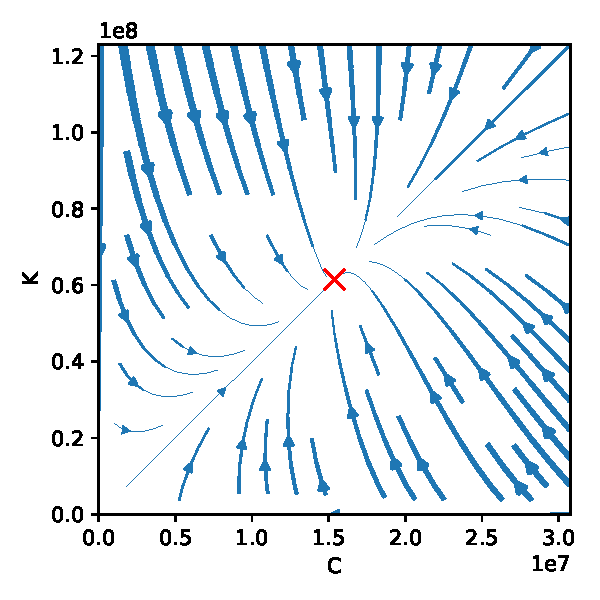
\includegraphics[width = .55 \textwidth]{./figures/phasespace.pdf}
	\caption{Phase space plot of equations \eqref{eq:full_clean_ca} \label{phase_space_plot}}
\end{wrapfigure}
Along the same lines, we can treat the case of a full clean economy (assuming that the fossil resource is depleted, or the households have for some other reason decided to only invest in clean capital $K_c$). \\
In this case, the equations for capital and knowledge accumulation are
\begin{align}
	\dot{K}_c &= s b_c L^{\alpha} K_c^{\beta} C^\gamma - \delta K_c \\
	\dot{C} &= b_c L^\alpha K_c^\beta C^\gamma - \chi C
	\label{eq:full_clean_ca}
\end{align}
Assuming that $\alpha + \beta$ = 1, with equal elasticities for capital and labor e.g. $\alpha = \beta$, the stationary points of the system are 
\begin{equation}
  (K_c^*, C^*) = (0,0), \left( \left( \frac{\chi s}{\delta} \right) \left( \frac{s b_c^2 L}{\delta \chi} \right)^{\frac{1}{1-2\gamma}}, \left( \frac{s b_c^2 L}{\delta \chi} \right)^{\frac{1}{1-2 \gamma}}  \right)
	\label{stationary_points}
\end{equation}
where the first one is non hyperbolic and the second one is stable which can be seen in the phase space plot in fig \ref{phase_space_plot} and the corresponding Jacobian
\begin{equation}
	J_{(K_c^*,C^*)} = 
		\begin{pmatrix}
			-\frac{1}{2}\delta & \frac{1}{2}\gamma s \delta \\
			\frac{\delta}{2 s} & \delta \left( \frac{\gamma}{2}-1 \right)
		\end{pmatrix}
	\label{eq:learning_jacobian}
\end{equation}
whose Eigenvalues are strictly negative:
\begin{equation}
  \lambda_{1,2} = \frac{\delta}{2}(\gamma-1), \quad -\delta.
	\label{eq:learning_eigenvalues}
\end{equation}
The phase space plot in fig. \ref{phase_space_plot} also suggests that there is a trajectory that satisfies 
\begin{equation}
	\frac{K_c(t)}{C(t)} = \frac{K^*_c}{C^*}
\end{equation}
meaning, one has to find a solution to the following ode:
\begin{equation}
	\dot{K}_c = s^{1-\frac{\gamma}{2}} b_c L_c^{\frac{1}{2}}K_c^{\frac{1}{2}(1-\gamma)} - \delta K_c
	\label{eq:learning_trajectory_ode}
\end{equation}
which can be done by means of separation of variables, resulting in
\begin{equation}
  K_c(t) = \left( s^{1-\frac{\gamma}{2}}\frac{b_c L^{\frac{1}{2}}}{\delta} + \exp\left[ (t_0-t) \frac{\delta (1-\gamma)}{2} \right] \right)^{\frac{2}{1-\gamma}}.
	\label{eq:learning_trajectory_solution}
\end{equation}
So, the system approaches its equilibrium approxitely exponentially from below, on a timescale that is given by
\begin{equation}
	t_c^* = \frac{2}{\delta(1-\gamma)}
	\label{eq_learning_equilibrium_timescale}.
\end{equation}
Assuming the same capital depreciation rate for clean capital as for dirty capital previously, together with $\gamma = 1/4$ (as suggested by Jobst Heitzig), the timescale for clean capital accumulation is $t^*_c \approx 53 y$.


\subsubsection{Fossil resource depletion}
\label{sec:resource_depletion}

\begin{wrapfigure}[16]{o}{.45 \textwidth}
	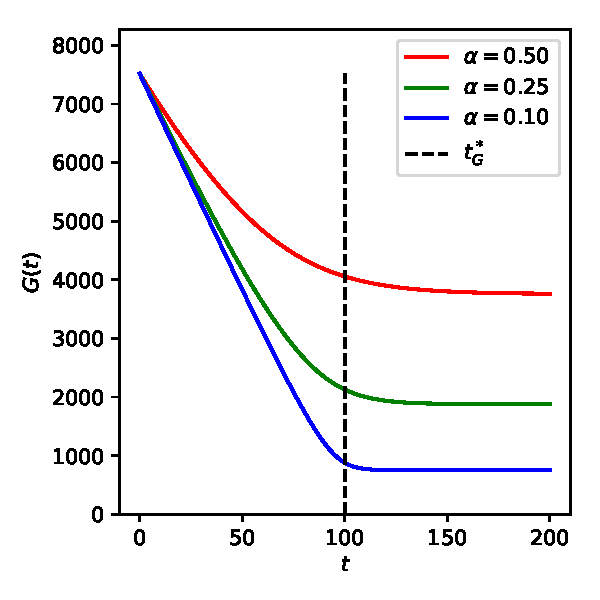
\includegraphics[width = .9 \textwidth]{./figures/g_depletion.pdf}
	\caption{Resource depletion in a full dirty economy as described by eq. \eqref{eq:resource_deprec_approx}. The dashed line marks the approximate resource depletion time $t^*_G$. \label{fig:g_depletion}}
\end{wrapfigure}
For this analysis, we assume a full dirty economy like in \ref{sec:full_dirty_economy}. In addition, we assume that we can separate the timescales of resource depletion and dirty capital accumulation, e.g. we assume that dirty capital accumulation happens fast compared to fossil resource depletion such that we can approximate $K_d(t)$ with eq. \ref{eq:full_dirty_capital_equilibrium_values}. Consequently, the ode for fossil resource depletion is given by
\begin{align}
	\dot{G} &= -R \nonumber \\
        &= -\frac{b_d}{e}P^{\pi}K_d^{*\ \kappa_d} \nonumber \\
	&= - \frac{b_d}{e}L^{\alpha}\left(L^{\alpha} \frac{s}{\delta}b_d\left( 1-\frac{b_R}{e}\left( \frac{G_0}{G(t)} \right)^2 \right) \right)^{\frac{\beta_d}{1-\beta_d}}
	\label{eq:resource_deprec_approx}
\end{align}
This means, that unsurprisingly, $G$ converges to a stable fix point $G^* = \sqrt{b_R/e}\ G_0$. Separating variables and substituting $g = G/G_0$ and $\varepsilon = \sqrt{b_R/e}$, the transient dynamic is given by
\begin{equation}
	\int_1^{g(t)} \frac{{\mathrm d} g'}{1 - \varepsilon^2/g'^2} = - \frac{s b_d^2 P}{e \delta G_0} \ t
	\label{eq:resource_transient_integral}
\end{equation}
To get a rough estimate of the time that it takes for the resource to deplete, we assume that $\varepsilon << 1$ and consequently for the most time, $\varepsilon^2/g'^2 << 1$.
This means, that the integrand of the lhs.\ in eq.~\eqref{eq:resource_transient_integral} can be approximated by
\begin{equation}
	\int_1^{g(t)}1+\frac{\varepsilon^2}{g'^2} {\mathrm d}g' = \left[ g' - \frac{\varepsilon^2}{g'} \right]_1^{g(t)} = g(t) - \frac{\varepsilon^2}{g(t)} -1+\varepsilon^2.
	\label{eq:resource_transient_solution}
\end{equation}
This results in the implicit approximate solution:
\begin{equation}
  g(t) - \frac{\varepsilon^2}{g(t)} = 1 -\varepsilon^2 - \frac{s b_d^2 P}{e \delta G_0} \ t.
	\label{eq:resource_transient_solution2}
\end{equation}
According to this approximate solution, $g$ reaches $\alpha$ after a finite time $t^*_G$, which I use as the timescale for resource depletion:
\begin{equation}
	t^*_G = G_0\frac{e \delta}{s P b_d^2}\left( 1-\frac{b_R}{e} \right)
	\label{eq:resource_depletion_time}
\end{equation}
Figure \ref{fig:g_depletion} shows this resource depletion time in comparison to the numerical solution from eq. \ref{eq:resource_deprec_approx} for different values of $\alpha$ to give an impression of the goodness of the approximation. \\

There are different estimates for the depletion time of fossil resources ranging from approximately 60 years for crude oil to 100 years for gas and 200 years for coal.
So, we assume $t^*_G \approx 100y$. Using this, the initial resource stock $G_0$, the total population, the integrated world BIP (with an assumed growth rate of 2\%p.a.) we could get approximate estimates for $e$ and a relation of $b_d$ to  $b_R$.

% I use 2015 as the base year for my estimates. To estimate $e$ I use World GDP according to the World Bank database CITE ($75.037 \ 10^{12}$ \$) and world primary energy supply according to the BP statistical review of world energy ($13 \ 647$ Mtoe).
% Accordingly, $e$ is estimated at
% \begin{equation}
%   e \approx \frac{75.037 \; 10^{12} \; \$}{13.647 \; 10^9 \; \rm{toe}} = 5.5 \ 10^3 \left[ \frac{\$}{\rm{toe}} \right]
%   \label{ep:estimate_e}
% \end{equation}

\subsubsection{Opinion spreading in the adaptive voter model}
A common way to describe the dynamics of the adaptive voter model in terms of macroscopic variables is the pair approgammamation.
For simplicity, lets assume a system with two possible opinions $A$ and $B$, on a network with $N$ nodes and $K$ edges.
We describe the model using a vector $(x, y, z)^T$:
\begin{equation}
	x = \frac{[A]-[B]}{N}, \quad y = \frac{[AA]-[BB]}{K}, \quad z = \frac{[AB]}{K}
	\label{avm_variables}
\end{equation}
There are four possible events in the system
\begin{itemize}
	\item 1. an A node rewiring,
	\item 2. a B node rewiring,
	\item 3. an A node adapting a B node and 
	\item 4. a B node adapting an A node.
\end{itemize}
The probabilities for these events to happen are
\begin{align}
	p_1 &= \varphi\frac{z(1+x)}{2(1+y)}, \quad p_2 = \varphi \frac{z (1-x)}{2(1-y)} \\
	p_3 &= (1-\varphi)\frac{z(1+x)}{2(1+y)}1/2({\mathrm tanh}(\Delta I)-1),\\
	p_4 &= (1-\varphi)\frac{z(1-x)}{2(1-y)}1/2({\mathrm tanh}(-\Delta I)-1)
	\label{avm_event_ps}
\end{align}
and their influence on the state vector $s = (x, y, z)^T$ are $s' = s + s_i$ with $s_i$ one of the following:
\begin{align}
	s_1 &= \colvec{3}{0}{1}{-1}, \quad s_3 = \colvec{3}{-2}{-2k\frac{1+y}{1+x}}{-1+2k\frac{1-y-2z}{1-x}-\frac{1-y-2z}{1-y}}\\ 
	s_2 &= \colvec{3}{0}{-1}{-1}, \quad s_4 = \colvec{3}{2}{2k\frac{1+y}{1+x}}{-1+2k\frac{1-y-2z}{1-x}+\frac{1-y-2z}{1-y}}
	\label{avm_event_effects}
\end{align}
Such that in the limit for large N, one gets deterministic equations for $x$, $y$ and $z$:
\begin{align}
	\frac{\dot{x}}{\tau} =& -(1-\varphi)\frac{z}{2}\frac{1-x}{1-y}({\mathrm tanh}(\Delta I)-1) + (1-\varphi)\frac{z}{2}\frac{1+x}{1+y}({\mathrm tanh}(-\Delta I)-1) \\
\frac{\dot{y}}{\tau} =& \quad \varphi\frac{z}{2}\left( \frac{1+x}{1+y} + \frac{1-x}{1-y} \right) + (1-\varphi)kz\left( {\mathrm tanh}(-\Delta I) - {\mathrm tanh}(\Delta I) \right) \\
	\frac{\dot{z}}{\tau} =& -\varphi\frac{z}{2}\left( \frac{1+x}{1+y} + \frac{1-x}{1-y} \right) \nonumber \\
	& + (1-\varphi)\frac{z}{2} \left[ \frac{1+x}{1+y} \frac{1}{2}({\mathrm tanh}(\Delta I)-1) \left( (1+y-2z)\left( \frac{2k}{1+x}-\frac{1}{1+y} \right)-1 \right) \right. \nonumber \\
	& \hspace{1.9 cm} + \left.\frac{1-x}{1-y}\frac{1}{2}({\mathrm tanh}(-\Delta I)-1)\left( (1-y-2z)\left( \frac{2k}{1-x}-\frac{1}{1-y} \right)-1 \right)  \right]
	\label{avm_ode}
\end{align}
assuming that the income difference $\Delta I$ between different cue orders is sufficiently large, this can be reduced to
\begin{align}
	\frac{\dot{x}}{\tau} =& -(1-\varphi)\frac{z}{2}\frac{1-x}{1-y} \\
\frac{\dot{y}}{\tau} =& \quad \varphi\frac{z}{2}\left( \frac{1+x}{1+y} + \frac{1-x}{1-y} \right) + (1-\varphi)kz \\
	\frac{\dot{z}}{\tau} =& -\varphi\frac{z}{2}\left( \frac{1+x}{1+y} + \frac{1-x}{1-y} \right) \nonumber \\
	& + (1-\varphi)\frac{z}{2} \left[ \frac{1+x}{1+y} \left( (1+y-2z)\left( \frac{2k}{1+x}-\frac{1}{1+y} \right)-1 \right) \right]
	\label{avm_ode_reduced}
\end{align}
and from this we see, that the timescale for $x$ to reach its equilibrium values is roughly 
\begin{equation}
	t_a^* = \tau(1-\varphi)
	\label{avm_timescale}
\end{equation}
Since, at least according to my impression, people don't really change their minds or make new friends too often, I propose keeping this timescale between $1<t_a^*<10$ years.

\section{Preliminary Results}  

To investigate the full dynamics of the model, I conducted different numerical experiments. For these experiments, I used the following parameter values if not state otherwise:

\begin{table}[t] 
	\centering
	\begin{tabular}{r|l}
		Parameter & Default Value \\\hline
		$\alpha$ & 1/2 \\
		$\beta_c$ & 1/2 \\
		$\beta_d$ & 1/2 \\
                $\gamma$ & 1/4 \\
		$b_c$ & 1 \\
		$b_d$ & 1.2 \\
		$b_R$ & 1 \\
		$e$ & 100 \\
		$s$ & 0.23 \\
		$\delta $ & 0.06 \\
		$L$ & 500 \\
		$G_0$ & $\sim$ 35000 \\
	\end{tabular}
	\caption{Parameter values for numerical studies in arbitrary units.}
	\label{tab:parameter_values}
\end{table} 
Since I did not yet find a reliable estimate for $\varepsilon = \sqrt{b_R/e}$, I will conduct experiments for two different values, to point out any qualitative differences, that there might be.

To separate the effects of the adaptive voter dynamic and the heuristic decision making in the model, I conducted separate studies for only the dynamic voter dynamics, only the heuristic decision making and the combination of both effects. \\
Since I am interested in the transition from a dirty to a clean economy, I started the experiment with an equilibrium state with infinite fossil resource supply.\\

\textit{Note that in the first series of experiments, there is no learning yet, e.g. $C \equiv 0$.}

\subsection{Adaptive Voter Experiment}
For the adaptive voter experiment the only possible cues were [0] and [1] such that the only way for changes in investment decisions were imitation of neighbors behavior.
The vertical grey lines show the time at which two thirds of households have opted for investment in the clean sector, assuming that this would be the point when shutting down the dirty sector would be opportune for a policy maker. The background coloring shows the proportion of max.\ economically extractable fossil resources still left in the ground at that point.
\subsubsection{Decisions}
\begin{figure}[t]
	\centering
%	\includegraphics[width = \textwidth]{divestdata/X5o2_Dirty_Clean_Transition_No_TTB/results_N/decisions'alpha'=0o1.pdf}
	\caption{Fraction of households investing in clean capital for $\alpha=0.1$. The vertical grey lines show the time at which two thirds of households have opted for investment in the clean sector, assuming that this would be the point when shutting down the dirty sector would be opportune. }
\end{figure}
\begin{figure}[t]
	\centering
%	\includegraphics[width = \linewidth]{divestdata/X5o2_Dirty_Clean_Transition_No_TTB/results_N/decisions'alpha'=0o05.pdf}
	\caption{Fraction of households investing in clean capital for $\alpha=0.05$. The vertical grey lines show the time at which two thirds of households have opted for investment in the clean sector, assuming that this would be the point when shutting down the dirty sector would be opportune. }

\end{figure}
\subsubsection{Capital Rates}
\begin{figure}[t]
	\centering
%	\includegraphics[width = \linewidth]{divestdata/X5o2_Dirty_Clean_Transition_No_TTB/results_N/capital_rates'alpha'=0o1.pdf}
	\caption{Development of Capital rates for $\alpha=0.1$, $r_c$ is blue, $r_d$ is red. Background color indicates the fraction of economically useful fossil resource that is left in the ground as two thirds of households opt for clean investment.}
	\label{5o2_3}
\end{figure}

\begin{figure}[t]
	\centering
%	\includegraphics[width = \linewidth]{divestdata/X5o2_Dirty_Clean_Transition_No_TTB/results_N/capital_rates'alpha'=0o05.pdf}
	\caption{Development of Capital rates for $\alpha=0.05$, $r_c$ is blue, $r_d$ is red. Background color indicates the fraction of economically useful fossil resource that is left in the ground as two thirds of households opt for clean investment.}
	\label{5o2_4}
\end{figure}
\subsubsection{Market Shares}
\begin{figure}[t]
	\centering
%	\includegraphics[width = \linewidth]{divestdata/X5o2_Dirty_Clean_Transition_No_TTB/results_N/market_shares'alpha'=0o1.pdf}
	\caption{Development of market shares for $\alpha=0.1$}

\end{figure}

\begin{figure}[t]
	\centering
%	\includegraphics[width = \linewidth]{divestdata/X5o2_Dirty_Clean_Transition_No_TTB/results_N/market_shares'alpha'=0o05.pdf}
	\caption{Development of market shares for $\alpha=0.05$}

\end{figure}
Higher alpha apparently leads to earlier transitions from dirty to clean investment.
Comparing figures~\ref{5o2_3} and~\ref{5o2_4} it appears, that higher $\alpha$ leads to higher spikes in the clean capital rent $r_c$ during the transition. This suggest access demand for clean capital that is not supplied by the households. This can be explained by the relative timescales of the resource depletion and opinion spreading resulting in delayed adaptation of opinion prevalence to the changed fitness of the respective opinions.\\
So, apparently, increasing $\alpha$ leads to increasingly abrupt transition with lower fraction of resource remaining in the ground. Also, as expected, higher $\varphi$ leads to slower spreading of successful strategies up to the point where strategies can only be changed through noise/random strategy change. \\
This also shows, that the qualitative signature of the fragmentation transition persists even with noise prevalent in the system.

\subsection{Heuristic Decisions Experiment}

This experiment evaluates the model dynamics for fixed shares of cue orders. There is no rewiring or imitation, just economic dynamics and Heuristic decision making of households according to the cue orders that they have been assigned to in the initial conditions.
Choice of initial conditions for this experiment was somewhat hacky, since 
\begin{itemize}
	\item With cues that take neighbors decisions into account (cue 4 in our example), the clustering in the network of households has considerable influence on the decision making.
	\item I haven't found a way to reproduce the clustering of same opinions that is produced by the adaptive voter model whilst holding the fraction of different opinions constant. 
\end{itemize}
To nevertheless imitate the clustering of similar opinions in the initial conditions, I modified the initial Erd\H{o}s-R\'enyi random graph such that a fraction $\varphi$ of the link in between different opinions were replaced by links between households of equal opinions. 
\par
Figure~\ref{5o3_1} shows that - especially with high shares of cue orders depending on neighbors decisions - increased clustering leads to inhibition of successful investment decision making. Somewhat unsurprisingly, there is some mixtures of cue orders where clean investment decisions are maximal for intermediate clustering of same opinions.
\subsubsection{Decisions}
\begin{figure}[t]
	\centering
%	\includegraphics[width = \linewidth]{divestdata/X5o3_Types_Transition/results_N/decisions'alpha'=0o1.pdf}
	\caption{Fraction of households investing in clean capital for $\alpha=0.1$. The fractions of households with different cue orders investing in either clean or dirty capital are color coded.}
	\label{5o3_1}
\end{figure}
\begin{figure}[t]
	\centering
%	\includegraphics[width = \linewidth]{divestdata/X5o3_Types_Transition/results_N/decisions'alpha'=0o05.pdf}
	\caption{Fraction of households investing in clean capital for $\alpha=0.05$. The fractions of households with different cue orders investing in either clean or dirty capital are color coded.}
	\label{5o3_2}
\end{figure} 
\subsubsection{Capital Rates}
\begin{figure}[t]
	\centering
%	\includegraphics[width = \linewidth]{divestdata/X5o3_Types_Transition/results_N/capital_rates'alpha'=0o1.pdf}
	\caption{Development of Capital rates for $\alpha=0.1$, $r_c$ is blue, $r_d$ is red. Background color indicates the fraction of economically useful fossil resource that is left in the ground as two thirds of households opt for clean investment.}
	\label{5o3_3}
\end{figure}

\begin{figure}[t]
	\centering
%	\includegraphics[width = \linewidth]{divestdata/X5o3_Types_Transition/results_N/capital_rates'alpha'=0o05.pdf}
	\caption{Development of Capital rates for $\alpha=0.05$, $r_c$ is blue, $r_d$ is red. Background color indicates the fraction of economically useful fossil resource that is left in the ground as two thirds of households opt for clean investment.}

\end{figure}
\subsubsection{Market Shares}
\begin{figure}[t]
	\centering
%	\includegraphics[width = \linewidth]{divestdata/X5o3_Types_Transition/results_N/market_shares'alpha'=0o1.pdf}
	\caption{Development of market shares for $\alpha=0.1$, $Y_c$ is blue, $Y_d$ is red.}

\end{figure}

\begin{figure}[t]
	\centering
%	\includegraphics[width = \linewidth]{divestdata/X5o3_Types_Transition/results_N/market_shares'alpha'=0o05.pdf}
	\caption{Development of market shares for $\alpha=0.05$, $Y_c$ is blue, $Y_d$ is red.}

\end{figure}


\subsection{Full Model}
This experiment combines the effects of rewiring and imitation of cue orders and Heuristic decision making of households. Consequently, the decision to invest in clean capital spreads much quicker amongst households. This can be viewed from different angles.
\begin{itemize}
	\item Several cue orders lead to successful investment decisions in both economic regimes. They can be viewed as resilient in a changing fitness landscape.
	\item Cue orders that rely on the investment decision of neighbors tap into the `wisdom of the crowd'. This only works if households with different opinions are sufficiently connected. Otherwise, clusters of households relying on each others decisions stabilize one another (this can be seen for instance in figure~\ref{5o3_1} and~\ref{5o3_2})
\end{itemize}

\begin{figure}[t]
	\centering
%	\includegraphics[width = \linewidth]{divestdata/X5o2_Dirty_Clean_Transition/results_N/decisions'alpha'=0o1.pdf}
	\caption{Fraction of households investing in clean capital for $\alpha=0.1$. The fractions of households with different cue orders investing in either clean or dirty capital are color coded.}
	\label{5o2_1}
\end{figure}
\begin{figure}[t]
	\centering
%	\includegraphics[width = \linewidth]{divestdata/X5o2_Dirty_Clean_Transition/results_N/decisions'alpha'=0o05.pdf}
	\caption{Fraction of households investing in clean capital for $\alpha=0.05$. The fractions of households with different cue orders investing in either clean or dirty capital are color coded.}
	\label{5o2_2}
\end{figure}
\subsubsection{Capital Rates}
\begin{figure}[t]
	\centering
%	\includegraphics[width = \linewidth]{divestdata/X5o2_Dirty_Clean_Transition/results_N/capital_rates'alpha'=0o1.pdf}
	\caption{Development of Capital rates for $\alpha=0.1$, $r_c$ is blue, $r_d$ is red. Background color indicates the fraction of economically useful fossil resource that is left in the ground as two thirds of households opt for clean investment.}

\end{figure}

\begin{figure}[t]
	\centering
%	\includegraphics[width = \linewidth]{divestdata/X5o2_Dirty_Clean_Transition/results_N/capital_rates'alpha'=0o05.pdf}
	\caption{Development of Capital rates for $\alpha=0.05$, $r_c$ is blue, $r_d$ is red. Background color indicates the fraction of economically useful fossil resource that is left in the ground as two thirds of households opt for clean investment.}

\end{figure}
\subsubsection{Market Shares}
\begin{figure}[t]
	\centering
%	\includegraphics[width = \linewidth]{divestdata/X5o2_Dirty_Clean_Transition/results_N/market_shares'alpha'=0o1.pdf}
	\caption{Development of market shares for $\alpha=0.1$, $Y_c$ is blue, $Y_d$ is red.}

\end{figure}

\begin{figure}[t]
	\centering
%	\includegraphics[width = \linewidth]{divestdata/X5o2_Dirty_Clean_Transition/results_N/market_shares'alpha'=0o05.pdf}
	\caption{Development of market shares for $\alpha=0.05$, $Y_c$ is blue, $Y_d$ is red.}

\end{figure}

\section{Outlook}
Next, I thought I'd implement `campaigners', green investors who are persistent in their opinion and who rewire not preferably to themselves but randomly to households of other opinions. Then I'd experiment on how many of these campaigners are necessary in order to tip the system to a qualified majority of clean investment for a given amount of resource staying in the ground. \\

Learning in the clean sector also seems to be a promising lead. This could result in a number of campaigners and/or explorative investors feeding the clean sector op to a point where it is competitive - making other investors follow their lead.

\subsection{Experiments with learning in the clean sector}

In the next series of experiments, I implemented learning in the clean sector as outlined in section~\ref{learning}.
Consequently, with the appropriate choice of parameters, the system becomes bistable with 
\begin{itemize}
	\item one stable state of high fossil resource use, low clean investment and small clean tech.\ knowledge stock,
	\item and one stable state with low fossil resource use, high clean investment and large clean tech.\ knowledge stock.
\end{itemize}
Choice of parameters for the economic system is the following:

\begin{table}[t] 
	\centering
	\begin{tabular}{r|l}
		Parameter & Default Value \\\hline
		$\kappa_c$ & 1/2 \\
		$\kappa_d$ & 1/2 \\
		$\pi$ & 1/2 \\
		$\xi$ & 1/4 \\
		$e$ & 100 \\
		$b_c$ & 0.4 \\
		$b_d$ & 1.2 \\
		$b_R$ & 1 \\
		$s$ & 0.23 \\
		$\delta $ & 0.06 \\
		$P$ & 500 \\
		$G_0$ & $\sim$ 35000 \\
	\end{tabular}
	\caption{Parameter values for numerical studies with learning in arbitrary units.}
	\label{tab:learning_parameter_values}
\end{table}

Choice of parameters for the network amongst households is $N=100$, $p=0.125$ with an Erd\H{o}s-R\'enyi random graph as initial configuration. 

Like before, the initial conditions for the experiment are an equilibrium dirty economy with abundant fossil resources. At the start of the experiment the fossil resource depletion is switched on.\

\begin{figure}[t]
	\centering
%	\includegraphics[width = \linewidth]{divestdata/X5o4_Dirty_Clean_Transition/results_N/decisions'alpha'=0o1.pdf}
	\caption{Fraction of households investing in clean capital with different households types marked by colors. $\alpha=0.1$.}
	\label{fig:learning_decisions0o1}
\end{figure}

\begin{figure}[t]
	\centering
%	\includegraphics[width = \linewidth]{divestdata/X5o4_Dirty_Clean_Transition/results_N/decisions'alpha'=0o05.pdf}
	\caption{Fraction of households investing in clean capital with different households types marked by colors. $\alpha=0.5$.}
	\label{fig:learning_decisions0o05}
\end{figure}
These figures serve well to differentiate between the part of the transition that stems from the decision making and the part that relies on the adaptive voter process.
The plots in the uppermost row of figure~\ref{fig:learning_decisions0o1} and~\ref{fig:learning_decisions0o05} show the effect of only the decision making process (since the adaptive voter dynamic is negligibly slow) in contrast to the plots on the two rows below, that include the effect of the adaptive voter process.\\

But looking at the transition in terms of economic variables, it becomes obvious that it is still mainly driven by the depletion of the fossil resource. This is most visible, if we look at the cost in the dirty sector in figure \ref{fig:learning_dirty_cost0o1} and \ref{fig:learning_dirty_cost0o05}.

\begin{figure}[t]
	\centering
%	\includegraphics[width = \linewidth]{./divestdata/X5o4_Dirty_Clean_Transition/results_N/dirty_costs'alpha'=0o1.pdf}
	\caption{Factor costs in the dirty sector for $\alpha = 0.1$. Solid gray vertical lines indicate the time of qualified majority of clean investment decisions, the transparent gray area marks the standard error of this mean and the dashed/dot dashed gray lines indicate the earliest/latest times of incident. Background colors indicate the fraction of the fossil resource that is still in the ground when the clean majority is reached.}
	\label{fig:learning_dirty_cost0o1}
\end{figure}
\begin{figure}[t]
	\centering
%	\includegraphics[width = \linewidth]{./divestdata/X5o4_Dirty_Clean_Transition/results_N/dirty_costs'alpha'=0o05.pdf}
	\caption{Same as fig.~\ref{fig:learning_dirty_cost0o1} but with $\alpha = 0.05$.}
	\label{fig:learning_dirty_cost0o05}
\end{figure}
On average, this point is reached when the cost of the fossil resource becomes comparable to the cost of other input factors, although there are cases, when this happens  significantly earlier (indicated by the dashed grey line). It would be interesting to look at the exact distribution of these incidents (TO DO).
From the comparison of these figures, it is apparent, that larger alpha (e.g.\ smaller fraction of the fossil resource economically extractable) leads to a larger fraction of the fossil resource remaining in the ground when a clean majority is reached. \textit{note, that this is not in absolute numbers but in relation to the fraction of resource that can be economically extracted}.
This might be due to the fact, that $\alpha$ also influences the difference in return rates from the different kinds of capital resulting in the dirty state of the economy being less `stable' (its basin of attraction becoming smaller and shallower?) such that the system has higher probability to `tip' over into its second (clean) stable state. \\

Maybe interesting to look into: Runs with large amount of fossil resources that are sufficient to sustain a dirty economy for some time, then get scarcer and scarcer until the system tips into the clean state. Look at the distribution of tipping times, maybe use early warning signs (from the fluctuation of clean capital and investment) to predict the probability of tipping depending on the remaining fossil resource.

\subsection{Experiments with a divestment/green investment campaign}
In this experiment, I want to look into the effect that a green investment campaign might have on the transition from a dirty to a clean state of the economic model.\\
The campaign is implemented as follows: In addition to the types of households that were used previously (as described in sec.~\ref{sec:oppinion_formation_and_decision_making}) there is an additional type that I call \textit{campaigner}. Campaigners have the following properties:
\begin{figure}[t]
	\centering
%	\includegraphics[width = \linewidth]{./divestdata/X5o5_Dirty_Clean_Transition/results_N/dirty_costs'alpha'=0o1.pdf}
	\caption{Factor costs in the dirty sector for $\alpha = 0.1$. Solid gray vertical lines indicate the time of qualified majority of clean investment decisions, the transparent gray area marks the standard error of this mean and the dashed/dot dashed gray lines indicate the earliest/latest times of incident. Background colors indicate the fraction of the fossil resource that is still in the ground when the clean majority is reached.}
	\label{fig:campaign_dirty_cost0o1}
\end{figure}
\begin{itemize}
	\item Campaigners persistently invest in clean capital,
	\item Campaigners value their integrity over capital income e.g.\ they do not imitate other households even if they have higher income (in other contexts this behavior is called zealotry),
	\item Other households may become part of the campaign by imitating a campaigner through the established adaptive voter mechanism.
\end{itemize}
\begin{figure}[t]
	\centering
%	\includegraphics[width = \linewidth]{./divestdata/X5o5_Dirty_Clean_Transition/results_N/dirty_costs'alpha'=0o05.pdf}
	\caption{Same as fig.~\ref{fig:campaign_dirty_cost0o1} but with $\alpha = 0.05$.}
	\label{fig:campaign_dirty_cost0o05}
\end{figure}


\begin{wrapfigure}[19]{i}{.55 \textwidth}
	\vspace{-.4 cm}
%	\includegraphics[width = 1 \textwidth]{./figures/remaining_reserves.png}
	\caption{Fraction of economically valuable fossil resources remaining in the ground at the point in time when a qualified clean majority is reached \label{fig:remaining_reserves}}
\end{wrapfigure}

Looking at the costs in the dirty sector again, it is apparent that the initial size of the campaign has significant influence on the transition towards clean investment.This influence is also shown in fig \ref{fig:remaining_reserves}. Although from this plot, no clean tendencies can be deduced except that increasing initial campaign size as well as decreasing rewiring probability both have positive influence on the remaining resources.
Also, with the campaign present, the value of $\alpha$ has larger influence on the resulting fraction of fossil resource staying in the ground. I suspect that this can be explained as follows: As speculated earlier, larger $\alpha$ leads to smaller basin of attraction of the dirty state of the economy. If at a given point in time a fraction of the households is made to invest in the clean sector, this poses a disturbance to the system. This disturbance is more likely to tip the system into its other state, if the barrier between these states is smaller. Additionally, due to learning in the clean sector, a starting investment makes return rates in this sector go up, which leads all households that invest according to trends in return rates to join in - multiplying the effect of the initial investment of the campaigners.\\
Since being a campaigner is an absorbing state in the opinion dynamic, it is clear that eventually all other opinions will vanish. The question is, at what rate this happens and when. Looking at the shares of different types of households in figures \ref{fig:campaign_decisions0o1} and \ref{fig:campaign_decisions0o05} one finds that the fraction of campaigners grows very slowly first and then explodes to leave all other types marginalized.\\
\begin{figure}[t]
	\centering
%	\includegraphics[width = \linewidth]{./divestdata/X5o5_Dirty_Clean_Transition/results_N/decisions'alpha'=0o1.pdf}
	\caption{Household investment decisions marked by household types. Thick red line marks the fraction of households investing in clean capital. The stacked colors below this line mark the fractions these decisions according to the types of household who made them. The stacked colors above the red line indicate the types of households investing in dirty capital. The area in mint green marks the fraction of households that are campaigners.}
	\label{fig:campaign_decisions0o1}
\end{figure}
\begin{figure}[t]
	\centering
%	\includegraphics[width = \linewidth]{./divestdata/X5o5_Dirty_Clean_Transition/results_N/decisions'alpha'=0o05.pdf}
	\caption{Same as fig.~\ref{fig:campaign_decisions0o1} but with $\alpha = 0.05$.}
	\label{fig:campaign_decisions0o05}
\end{figure}


